\documentclass[12pt,a4paper]{report}

\usepackage{geometry}
\usepackage{graphicx}
\usepackage{longtable}
\usepackage{pgfgantt}
\usepackage[dutch]{babel}
\usepackage{url}
\usepackage{pgf,pgfplots}
\usetikzlibrary{fit,calc}
\usepgfplotslibrary{external}

\geometry{a4paper}

\newcommand{\boxplot}[6]{%
	%#1: center, #2: median, #3: 1/4 quartile, #4: 3/4 quartile, #5: min, #6: max
	\filldraw[fill=white,line width=0.2mm] let \n{boxxl}={#1-0.1}, \n{boxxr}={#1+0.1} in (axis cs:\n{boxxl},#3) rectangle (axis cs:\n{boxxr},#4);   % draw the box
	\draw[line width=0.2mm, color=red] let \n{boxxl}={#1-0.1}, \n{boxxr}={#1+0.1} in (axis cs:\n{boxxl},#2) -- (axis cs:\n{boxxr},#2);             	% median
	\draw[line width=0.2mm] (axis cs:#1,#4) -- (axis cs:#1,#6);                                                                           							% bar up
	\draw[line width=0.2mm] let \n{whiskerl}={#1-0.025}, \n{whiskerr}={#1+0.025} in (axis cs:\n{whiskerl},#6) -- (axis cs:\n{whiskerr},#6);        % upper quartile
	\draw[line width=0.2mm] (axis cs:#1,#3) -- (axis cs:#1,#5);                                                                           							% bar down
	\draw[line width=0.2mm] let \n{whiskerl}={#1-0.025}, \n{whiskerr}={#1+0.025} in (axis cs:\n{whiskerl},#5) -- (axis cs:\n{whiskerr},#5);        % lower quartile
}

\title{P\&O Computerwetenschappen - Verslag}
\author{Team Platinum}

\begin{document}

\maketitle
\tableofcontents

\begin{abstract}
Tijdens de uitwerking van dit jaar-overschrijdend groepswerk, zullen wij een autonome robot bouwen met behulp van Lego Mindstorms. Voor de programmatie wordt beroep gedaan op Lejos, een Open Bron project dat een minimale JAVA virtuele machine heeft gemaakt die de plaats kan innemen van de standaard programmatie omgeving van Lego.

Naast de doelstelling om kennis te maken met het ontwikkelen van een autonome robot, willen we in dit project ook ervaring opdoen ivm het werken in team verband aan een middelgroot softwareproject. Hierbij zijn organisatie van werk, planning, analyse, architectuur,... belangrijke begrippen.

Parallel met het verplicht te volgen traject van meerdere demo sessies, kiezen we voor een traject waarbij het uiteindelijke doel van het project wordt voorop gesteld: een volledig onbekend traject autonoom afleggen. Hiertoe hebben we na een korte analyse interfaces afgesproken, waar beide trajecten zich aan houden, om een integratie mogelijk te maken.

\bigskip

(De samenvatting wordt verder aangevuld met belangrijke aspecten die tijdens het verdere verloop van het project naar voor treden.)

\end{abstract}

\chapter{Inleiding}

De tussentijdse demo sessies helpen om de technologie stapsgewijs te verkennen. Echter geen van deze tussenstappen is rechtstreeks inzetbaar bij het effectieve doel: het autonoom rijden van een onbekend traject.

We kiezen er voor om ons team op te splitsen en twee verschillende trajecten te volgen: \'e\'en dat zich toelegt op het optimaal implementeren van de tussentijdse opdrachten en \'e\'en dat er voor zorgt dat een volledige architectuur uitgewerkt wordt die ons zal toelaten om de eindopdracht optimaal te realiseren.

Op basis van een architectuur studie werden de componenten van de eindoplossing ge\"identificeerd. In een Work Breakdown Structure\footnote{\url{http://en.wikipedia.org/wiki/Work_breakdown_structure}} (WBS) werden vervolgens de deelstappen opgelijst, toegewezen aan verantwoordelijken en deadlines bepaald. Deze informatie vormde de basis voor een planning. De WBS en planning zijn opgenomen in respectievelijk bijlagen \ref{appendix:wbs} en \ref{appendix:planning}

\section{Architectuur}

De architectuur die we zullen implementeren in dit project richt zich op het realiseren van een robuuste oplossing. Echter niet alleen op het vlak van de autonome robot, maar ook op het volledige framework er rond dat we opbouwen op de PC. Figuur \ref{fig:architectuur} geeft de algemene architectuur weer. We belichten vervolgens de architectuur van uit het oogpunt van beide omgevingen waar de oplossing zal actief zijn: de robot en de PC.

\begin{figure}[htbp]
   \centering
   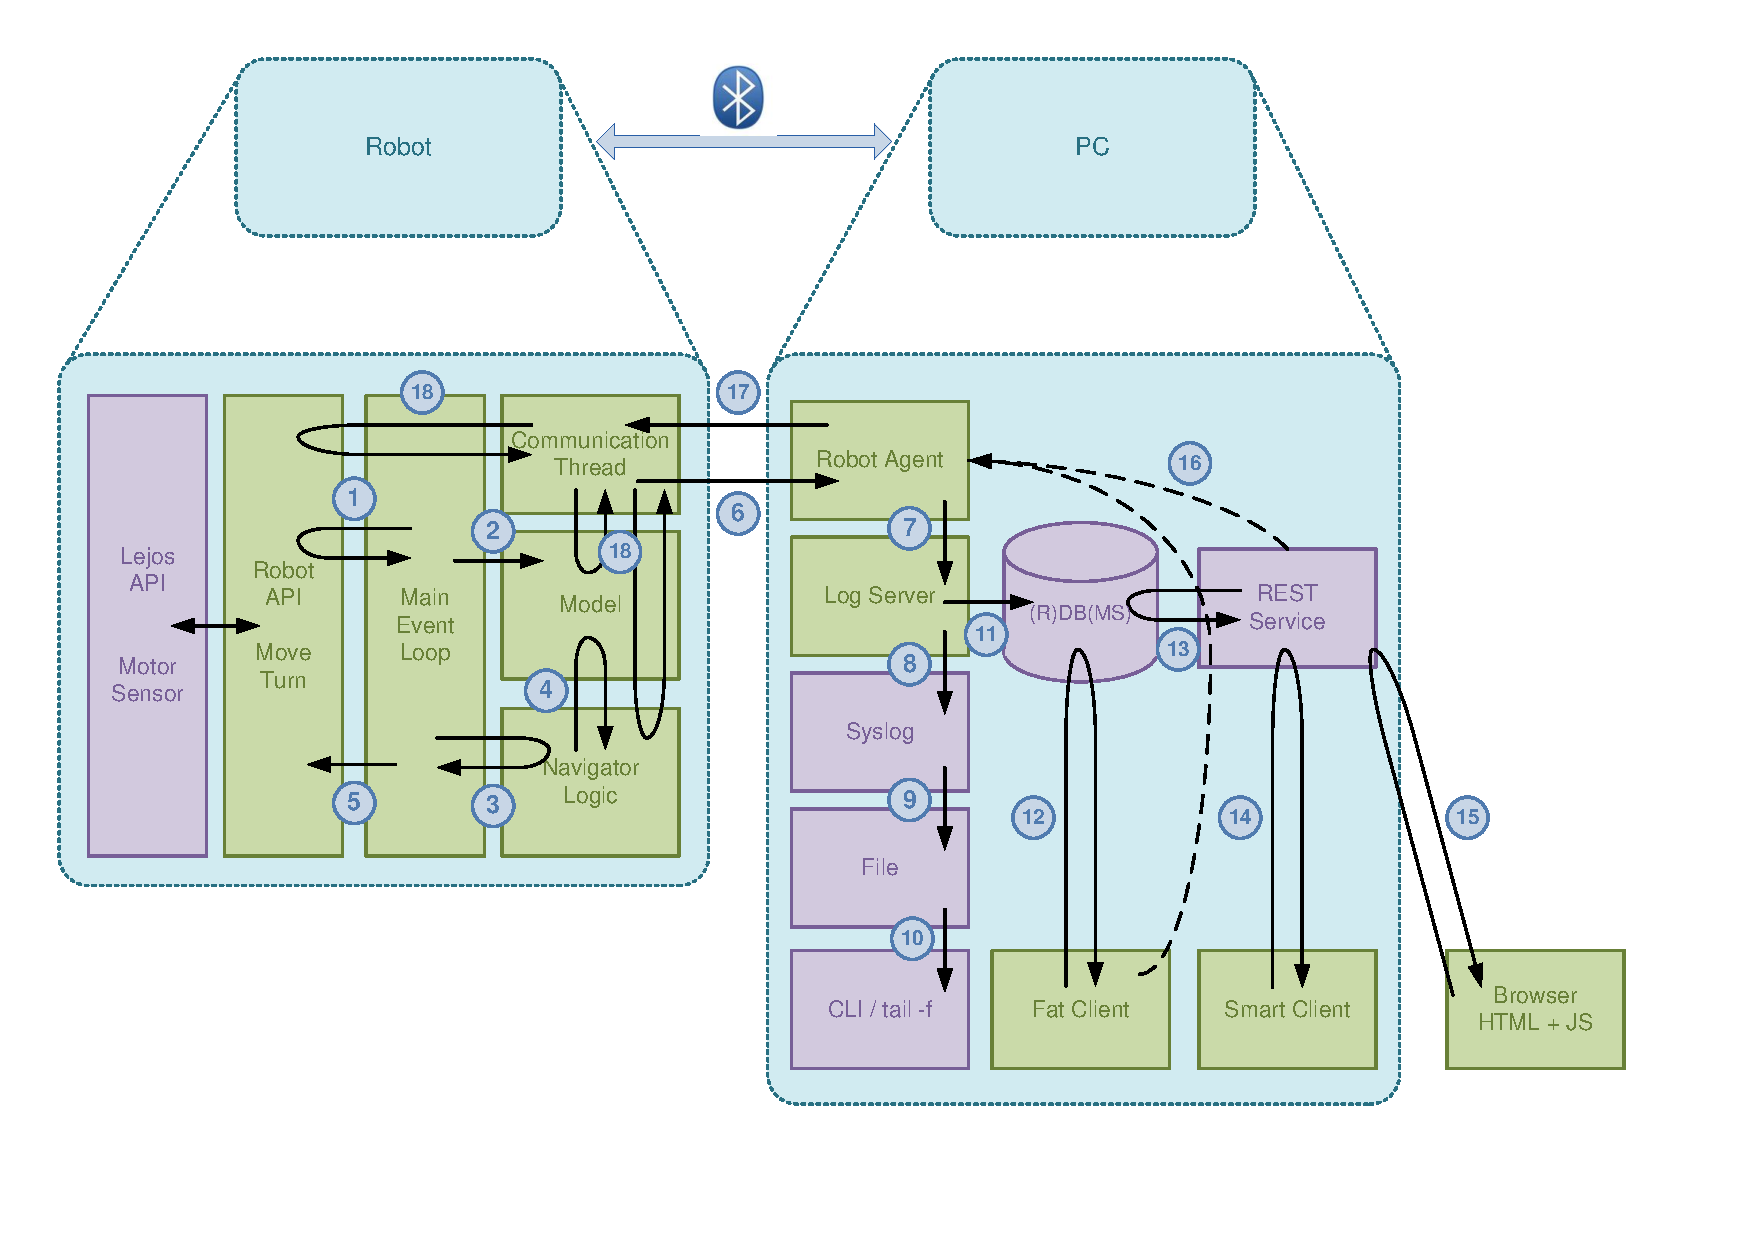
\includegraphics[width=200mm, angle=90]{resources/architectuur.pdf}
   \caption{Architectuur}
   \label{fig:architectuur}
\end{figure}

\subsection{Robot}

De robot biedt een technische API die toegang verleent tot de motoren en sensoren. We kiezen er voor om een eigen RobotAPI te cre\"eren die abstractie maakt van de technische API. Dit zal ons toelaten om een simulatieomgeving te bouwen met een andere implementatie van dezelfde interface. Zo'n simulatieomgeving zal ons vervolgens toelaten om de logica die moet ontwikkeld worden voor de eindoplossing onafhankelijk van de fysieke robot te testen. 

Een tweede belangrijke component binnen de robot, wordt de �Main Event Loop�\footnote{\url{http://en.wikipedia.org/wiki/Event_loop}}. We hergebruiken hier een term die uit de wereld van de grafische gebruikers interfaces komt, maar zeer goed weergeeft wat hier gebeurt. De Main Event Loop doorloopt eindeloos 5 stappen: 

\begin{enumerate}
\item haal gegevens op van alle sensoren
\item voed de gegevens in het model
\item ondervraag de navigator welke acties dienen ondernomen te worden
\item de navigator consulteert het model om de volgende acties te bepalen
\item voer de acties uit door middel van de robot API
\end{enumerate}

Het model is een interne voorstellingsvorm van de wereld waarin de robot zich begint. Aan het begin van de Event Loop, zal dit model leeg zijn, of eerder volledig onbekend. Gaandeweg zal op basis van de input van de sensoren dit model gevoed worden en zal een wereldbeeld ontstaan met verschillende graden van zekerheid.

De navigator consulteert vervolgens dit model om de volgende actie te bepalen en implementeert op deze manier het "doel" van de robot. Deze acties worden uitgedrukt in de taal van de RobotAPI en bestaan uit functionele opdrachten zoals beweeg $x$ meter vooruit of draai $x$ graden. De analogie met de copiloot/navigator gaat hier volledig op.

Naast de Main Event Loop, voorzien we een tweede onafhankelijke Event Loop, namelijk voor de communicatie met de PC. Deze geschiedt via Bluetooth. De redenen om deze gescheiden te houden zijn triviaal: enerzijds willen we de werking van de robot zelf niet onnodig in gevaar brengen met een proces dat kan falen. Anderzijds zal ook de frequentie waarop beide processen opereren niet gelijk lopen.

Een voorbeeld hiervan is de stroom van informatie die de lichtsensoren of sonar zullen aanbieden. Het volledig overzenden van deze gegevens kan eventueel niet mogelijk en niet wenselijk zijn.

\subsection{PC}

Op de PC wordt alle communicatie met de robot verzorgd langs een zgn. Robot Agent. We voorzien deze laag om de robuustheid van de oplossing te verhogen. Door het beperken van de synchrone code, verlagen we het risico dat externe factoren de communicatie met de robot verstoren. We denken hierbij aan het rechtstreeks koppelen van de communicatie aan een gebruikersinterface.

We zijn van mening dat het louter verzenden en visualiseren van informatie over de werking van de robot een verlies aan mogelijkheden zou betekenen. Onze strategie, met een simulatieomgeving, toont al snel aan dat deze informatie kan helpen bij het onderzoek naar optimale navigator-logica.

Aangezien we de informatie dus wensen te bewaren, willen we dit ook een centraal gegeven van onze architectuur maken. Opnieuw komt dit de robuustheid van de gehele oplossing ten goede. De focus zal komen te liggen op het optimaal opslaan van de gegevens. Het visualiseren ervan komt vervolgens neer op het opvragen ervan, wat opnieuw een asynchroon proces is.

Deze architectuur heeft enkele bijkomende gevolgen. Zo wordt het bvb. mogelijk om gegevens van meerdere sessies simultaan te bekijken of kan met meerdere en/of verschillende gebruikersinterfaces gewerkt worden. Ook kan voor de realisatie van deze architectuur beroep gedaan worden op enkele standaarden, waardoor het cre"eren van nieuwe code tot een minimum beperkt wordt.

Zo kan de Log Server ge"implementeert worden op basis van log4j\footnote{\url{http://logging.apache.org/log4j/}} en kan de aflevering van de inkomende communicatie volledig in configuratie gerealiseerd worden. De meest eenvoudige uitwerking kan bestaan uit het gebruiken van een syslog daemon, maar ook een relationele databank is triviaal.

Verschillende types clients kunnen de gegevens uit de databank visualiseren: een Fat Client\footnote{\url{http://en.wikipedia.org/wiki/Fat_client}} ligt voor de hand, maar ook een web-applicatie of REST\footnote{\url{http://en.wikipedia.org/wiki/Representational_state_transfer}} service zijn goede opties.

Deze laatste kan dan opnieuw gerealiseerd worden gebruikmakend van standaard componenten zoals de JBoss applicatie server\footnote{\url{http://www.jboss.org/jbossas}} en RESTeasy\footnote{\url{http://www.jboss.org/resteasy}}. Door middel van JSONP\footnote{\url{http://en.wikipedia.org/wiki/JSONP}} kan zelfs een streaming oplossing aan web-clients aangeboden worden.

\subsection{Interactie}

De architectuur (figuur \ref{fig:architectuur}) voorziet ook de mogelijkheid om commando's te sturen naar de robot. Aan de robot-kant zullen de meeste van de componenten handelingen registreren bij de communicatie component. Op deze manier kunnen de commando's door de communicatie component uitgevoerd worden op de geregistreerde handelingen op de componenten. Dit stelt ons in staat om op generieke manier interactief de software van de robot te ondervragen, zonder specifieke code te moeten voorzien.

\section{Functionele Analyse}

In de functionele analyse bepalen we in hoofdzaak de interfaces die gerespecteerd dienen te worden in de twee trajecten. Op basis van deze afspraken kunnen beide trajecten integreren en in elkaar opgaan.

Twee interfaces dienen zich aan: de Robot interface en de RobotAPI interface. De eerste bepaalt hier de robot opgebouwd en aangesproken kan worden door zijn omgeving. Dit kan een programma zijn dat op de robot uitgevoerd wordt, of dit kan onze simulatieomgeving zijn. Ook op niveau van de RobotAPI moet deze mogelijkheid beschikbaar zijn.

\begin{figure}[htbp]
   \centering
   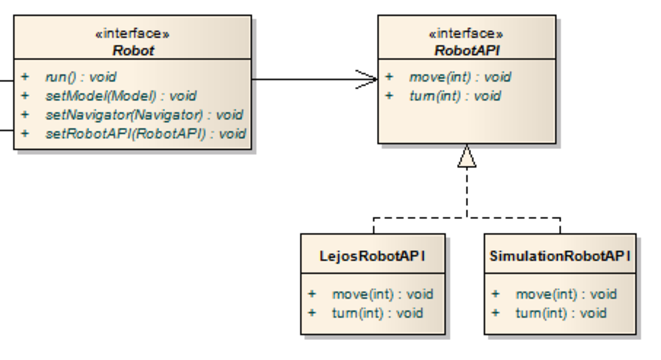
\includegraphics[width=100mm]{resources/robotapi.pdf}
    \caption{Robot \& RobotAPI}
   \label{fig:robotapi}
\end{figure}

De volledige klasse diagrammen zijn consulteerbaar in bijlage \ref{appendix:classdiagrams}.

\chapter{Demo 1: Veelhoek}

De doelstelling van de eerste demo is het rijden van een veelhoek op basis van het aantal hoeken en de lengte van een zijde. Precisie door middel van compensatie van de vast te stellen afwijkingen is hier van belang.

\section{De robot}

Het ontwerp van de robot voor de eerste opdracht is het basismodel van de Mindstorms kit die we ter beschikking kregen. Gegeven het korte tijdsbestek was het belangrijker om snel ervaring op te doen met de robot. Deze ervaring kan informatie verschaffen aan het lange termijn traject.
 
\section{De software}
 
De Lejos API biedt twee mogelijkheden om de motoren aan te sturen: op basis van tijd en op basis van de omwentelingen van de wielen. Intu\"itief waren we overtuigd dat de methode op basis van omwentelingen de meest betrouwbare moest zijn. Maar we moeten dit kunnen aantonen.

Wat betreft de rij-technische mogelijkheden, kiezen we voor twee onafhankelijke bewegingen: het rechtdoor rijden (vooruit of achteruit) en het ter plekke draaien. Dit is enerzijds een noodzaak voor de opdracht, maar is tevens de meest berekenbare methode.

In beide gevallen is er nog een parameter die bepalend kan zijn: de rotatiesnelheid. Ook deze zullen we in onze testen laten vari\"eren om een optimale verhouding te vinden.

\section{Testplan en resultaten}

\subsection{Omwentelingen}

De implementatie die omwentelingen telt is afhankelijk van de omtrek van de wielen. De theoretische omtrek van het wiel kan berekend worden op basis van de diameter (56mm) en bedraagt 175,93mm.

Naast de theoretische bepaling van de omtrek hebben we ook software voorzien die deze omtrek bepaalt op basis van een zgn. zelf-calibratie. Hierbij laten we de robot rijden, voorzien van een frontale druksensor, tot hij een obstakel raakt. Op dit ogenblik stop de robot. Vervolgens nemen we de blokkade weg en zal de robot na enkele seconden zelf verder rijden tot het volgende obstakel. Op basis van de getelde omwentelingen en de vaste afstand tussen beide obstakels, kan de robot vervolgens zelf exact de omtrek van het wiel bepalen.

De waarde die op deze manier werd vastgesteld was 175mm. We hebben deze gebruikt als initi\"ele waarde.

\subsubsection{Test 1: met een vaste snelheid verschillende afstanden rijden}

Voor deze test werd de snelheid ingesteld op 400 en werden afstanden van 20, 40, 60 en 80 cm gereden. Bij de uiteindelijke opdracht wordt er gereden op een parcours dat bestaat uit panelen van 80 bij 80 cm. De robot zal zelden grotere afstanden aan \'e\'en stuk rijden.

We lieten de robot telkens 5 maal de vooropgestelde afstand rijden en berekenden vervolgens de relatieve afwijkingen. De resultaten van deze test zijn opgenomen in figuur \ref{chart:test1}.

\begin{figure}
	\caption{Test 1 : Relatieve afwijking bij vaste snelheid}
	\label{chart:test1}
	\vspace{10pt}	
	\centering
	
	\tikzset{external/remake next}
	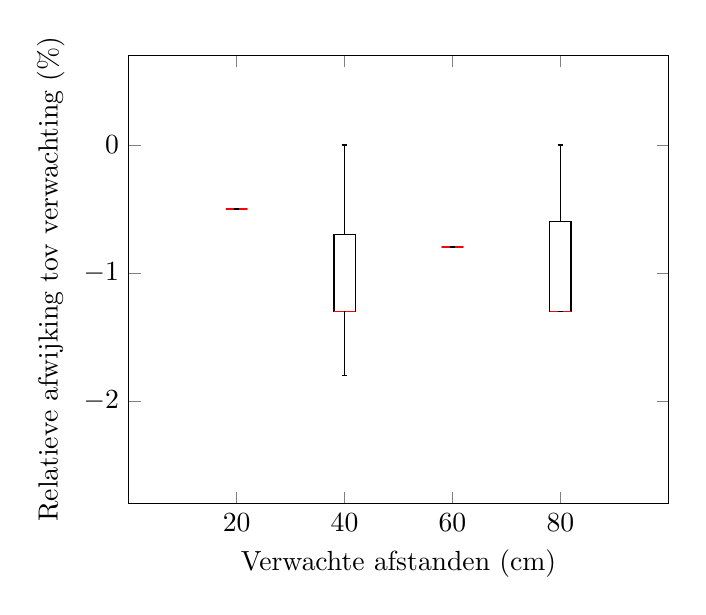
\begin{tikzpicture}
		\begin{axis}[xmin=0,xmax=5,ymin=-2.8, ymax=0.7,
			xtick={1,2,3,4,5},xticklabels={20,40,60,80},
	      		xlabel={Verwachte afstanden (cm)},
			ylabel={Relatieve afwijking tov verwachting (\%)},
			]
			%#1: center, #2: median, #3: 1/4 quartile, #4: 3/4 quartile, #5: min, #6: max
			\boxplot{1}{-0.5}{-0.5}{-0.5}{-0.5}{-0.5}
			\boxplot{2}{-1.3}{-1.3}{-0.7}{-1.8}{0}
			\boxplot{3}{-0.8}{-0.8}{-0.8}{-0.8}{-0.8}
			\boxplot{4}{-1.3}{-1.3}{-0.6}{-1.3}{0}
		\end{axis}
	\end{tikzpicture}
\end{figure}

Op basis van de resultaten, werd de wielomtrek met 1\% verkleind. Figuur \ref{chart:test1b} toont de resultaten van dezelfde test na de aanpassing.

\begin{figure}
	\caption{Test 1 : Resultaten na aanpassing wielomtrek met 1\%}
	\label{chart:test1b}
	\vspace{10pt}	
	\centering
	
	\tikzset{external/remake next}
	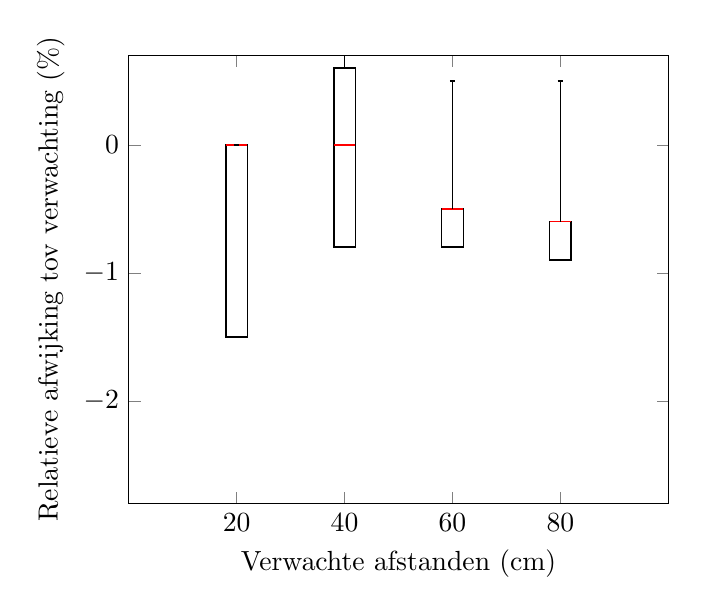
\begin{tikzpicture}
		\begin{axis}[xmin=0,xmax=5,ymin=-2.8, ymax=0.7,
			xtick={1,2,3,4,5},xticklabels={20,40,60,80},
	      		xlabel={Verwachte afstanden (cm)},
			ylabel={Relatieve afwijking tov verwachting (\%)},
			]
			%#1: center, #2: median, #3: 1/4 quartile, #4: 3/4 quartile, #5: min, #6: max
			\boxplot{1}{0}{-1.5}{0}{-1.5}{0}
			\boxplot{2}{0}{-0.8}{0.6}{-0.8}{0.8}
			\boxplot{3}{-0.5}{-0.8}{-0.5}{-0.8}{0.5}
			\boxplot{4}{-0.6}{-0.9}{-0.6}{-0.9}{0.5}
		\end{axis}
	\end{tikzpicture}
\end{figure}

\subsubsection{Test 2: een vaste afstand met verschillende snelheden}

Bij het uitvoeren van verkennende testen hadden we reeds vastgesteld dat het vertrekken, stoppen en de snelheid van de motoren een beduidende invloed hadden op de stabiliteit van de robot. Met deze tweede test willen we op zoek gaan naar een optimale snelheid/precisie verhouding.

We lieten de robot telkens 5 maal een afstand van 20cm afleggen bij vari�rende motorsnelheden: 125, 250, 500, 750 en 1000. Vervolgens  berekenden we de realtieve afwijking. De resultaten van deze test zijn opgenomen in figuur \ref{chart:test2}.

\begin{figure}
	\caption{Test 2 : Relatieve afwijking bij variabele snelheden}
	\label{chart:test2}
	\vspace{10pt}	
	\centering
	
	\tikzset{external/remake next}
	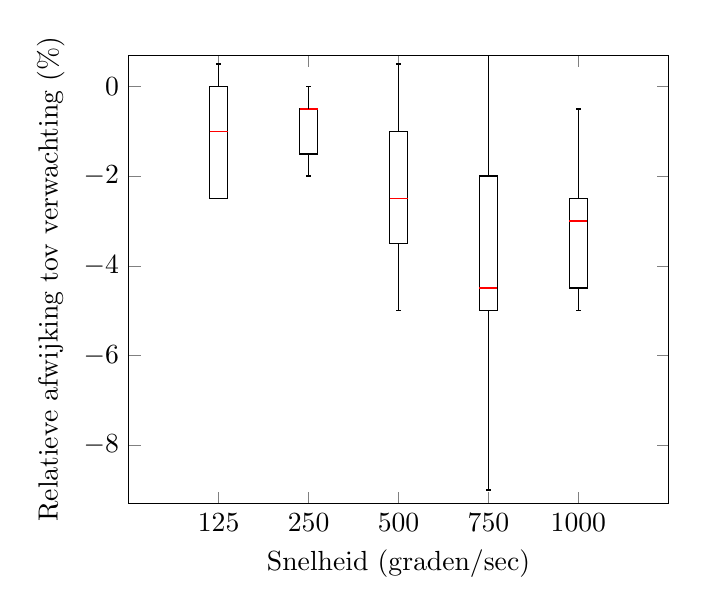
\begin{tikzpicture}
		\begin{axis}[xmin=0,xmax=6,ymin=-9.3, ymax=0.7,
			xtick={1,2,3,4,5,6},xticklabels={125,250,500,750,1000},
	      		xlabel={Snelheid (graden/sec)},
			ylabel={Relatieve afwijking tov verwachting (\%)},
			]
			%#1: center, #2: median, #3: 1/4 quartile, #4: 3/4 quartile, #5: min, #6: max
			\boxplot{1}{-1.0}{-2.5}{0}{-2.5}{0.5}
			\boxplot{2}{-0.5}{-1.5}{-0.5}{-2}{0}
			\boxplot{3}{-2.5}{-3.5}{-1.0}{-5.0}{0.5}
			\boxplot{4}{-4.5}{-5}{-2}{-9}{1.5}
			\boxplot{5}{-3.0}{-4.5}{-2.5}{-5}{-0.5}
		\end{axis}
	\end{tikzpicture}
\end{figure}

Uit de resultaten besloten we dat 250 graden per seconde ons de meest betrouwbare snelheid gaf.

Met deze snelheid werden vervolgens opnieuw verschillende afstanden gereden. De resultaten bevestigde de eerder gevonden foutenmarge van ongeveer 1\%.

Dat de kwaliteit van de Lego onderdelen van groot belang kan zijn, bleek toen het omwisselen van twee wielen een oplossing bleek te zijn voor een grote afwijking naar \'e\'en bepaalde kant.

\subsubsection{Test 3: hoeken}

Het ter plekke draaien is ook gebaseerd op de wielomtrek, echter nu in combinatie met de draaicirkel die bepaald wordt door de wielafstand.

Om de nauwkeurigheid van het ter plekke draaien te bepalen, lieten we de robot 5 maal een zelfde hoek draaien. Hierbij varieerden we de hoeken als volgt: 15, 30, 45, 60 en 90 graden. Opnieuw keken we naar de eindopgave. We verwachten niet dat we met de robot veel hoeken groter dan 90 graden gaan moeten maken. Voor de veelhoek-opdracht, is dit normaal niet het geval, met een spreekwoordelijke uitzondering voor een driehoek.

Ook voor deze test wilden we de parameter snelheid in beschouwing nemen. Uit de eerste resultaten bleek snel dat een snelheid hoger dan de eerder vastgestelde 250 graden per seconde niet accepteerbare afwijkingen opleverde. We hebben deze testen verder niet weerhouden.

De resultaten voor de verschillende hoeken zijn weergegeven in figuur \ref{chart:test3}.

\begin{figure}
	\caption{Test 3 : Relatieve afwijking bij vaste snelheid}
	\label{chart:test3}
	\vspace{10pt}	
	\centering
	
	\tikzset{external/remake next}
	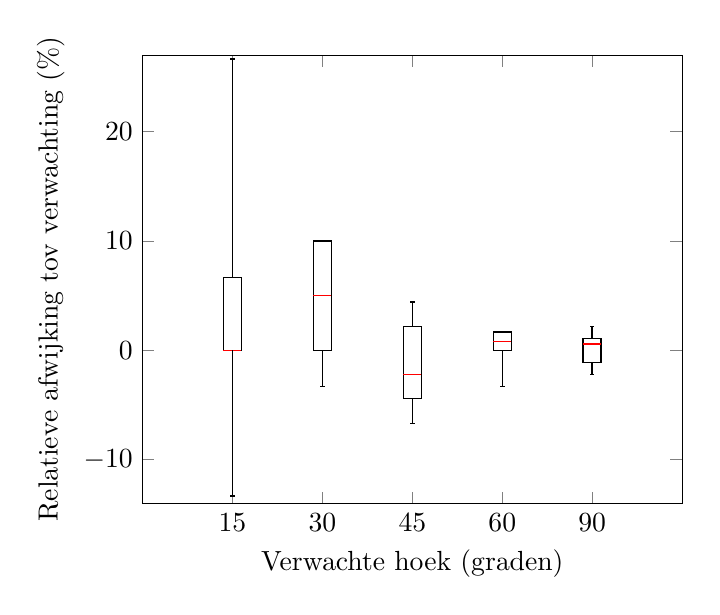
\begin{tikzpicture}
		\begin{axis}[xmin=0,xmax=6,ymin=-14.0, ymax=27,
			xtick={1,2,3,4,5,6},xticklabels={15,30,45,60,90},
	      		xlabel={Verwachte hoek (graden)},
			ylabel={Relatieve afwijking tov verwachting (\%)},
			]
			%#1: center, #2: median, #3: 1/4 quartile, #4: 3/4 quartile, #5: min, #6: max
			\boxplot{1}{0}{0}{6.67}{-13.3}{26.67}
			\boxplot{2}{5}{0}{10}{-3.3}{10}
			\boxplot{3}{-2.2}{-4.4}{2.2}{-6.7}{4.4}
			\boxplot{4}{0.8}{0}{1.7}{-3.3}{1.7}
			\boxplot{5}{0.6}{-1.1}{1.1}{-2.2}{2.2}
		\end{axis}
	\end{tikzpicture}
\end{figure}

De resultaten bevestigden het vermoeden dat de fout groter is bij kleinere hoeken. De resultaten bij 60 en 90 graden zijn dan weer positief met het oog op het rijden van een parcours met typisch die soort hoeken.

\subsubsection{Conclusie ivm omwentelingen}

Met een snelheid van 250 en een bijstelling van de omtrek van het wiel met 1\% zou de robot, volgens onze metingen vrij precies een willekeurige veelhoek moeten kunnen rijden.

Dit werd bevestigd bij het toepassen van deze implementatie voor het rijden van een veelhoek. Hierbij werden testen gedaan waarbij achtereenvolgens een 3, 4, 5, 6, 10 en 15-hoek werd gereden met een zijde van 20 of 30 cm. De 3, 4, 5 en 6-hoeken waren nagenoeg perfect. Bij de 10 en 15 hoek merkten we de (toen nog niet bijgewerkte) fout van 1\% op.

Figuur \ref{fig:resultsLargePolygons} toont het papier waarop we start en eindpunten aanduidden bij de grote veelhoeken en toont de afwijkingen van enkele metingen ten opzichte van het startpunt. De rode omtrek geeft de startpositie van de robot weer met het middelpunt aangegeven door het rode kruis. De zwarte kruisen zijn de middelpunten van 6 testen waarbij een 15 hoek met zijde 20 cm werd gereden.

\begin{figure}[htbp]
   \centering
   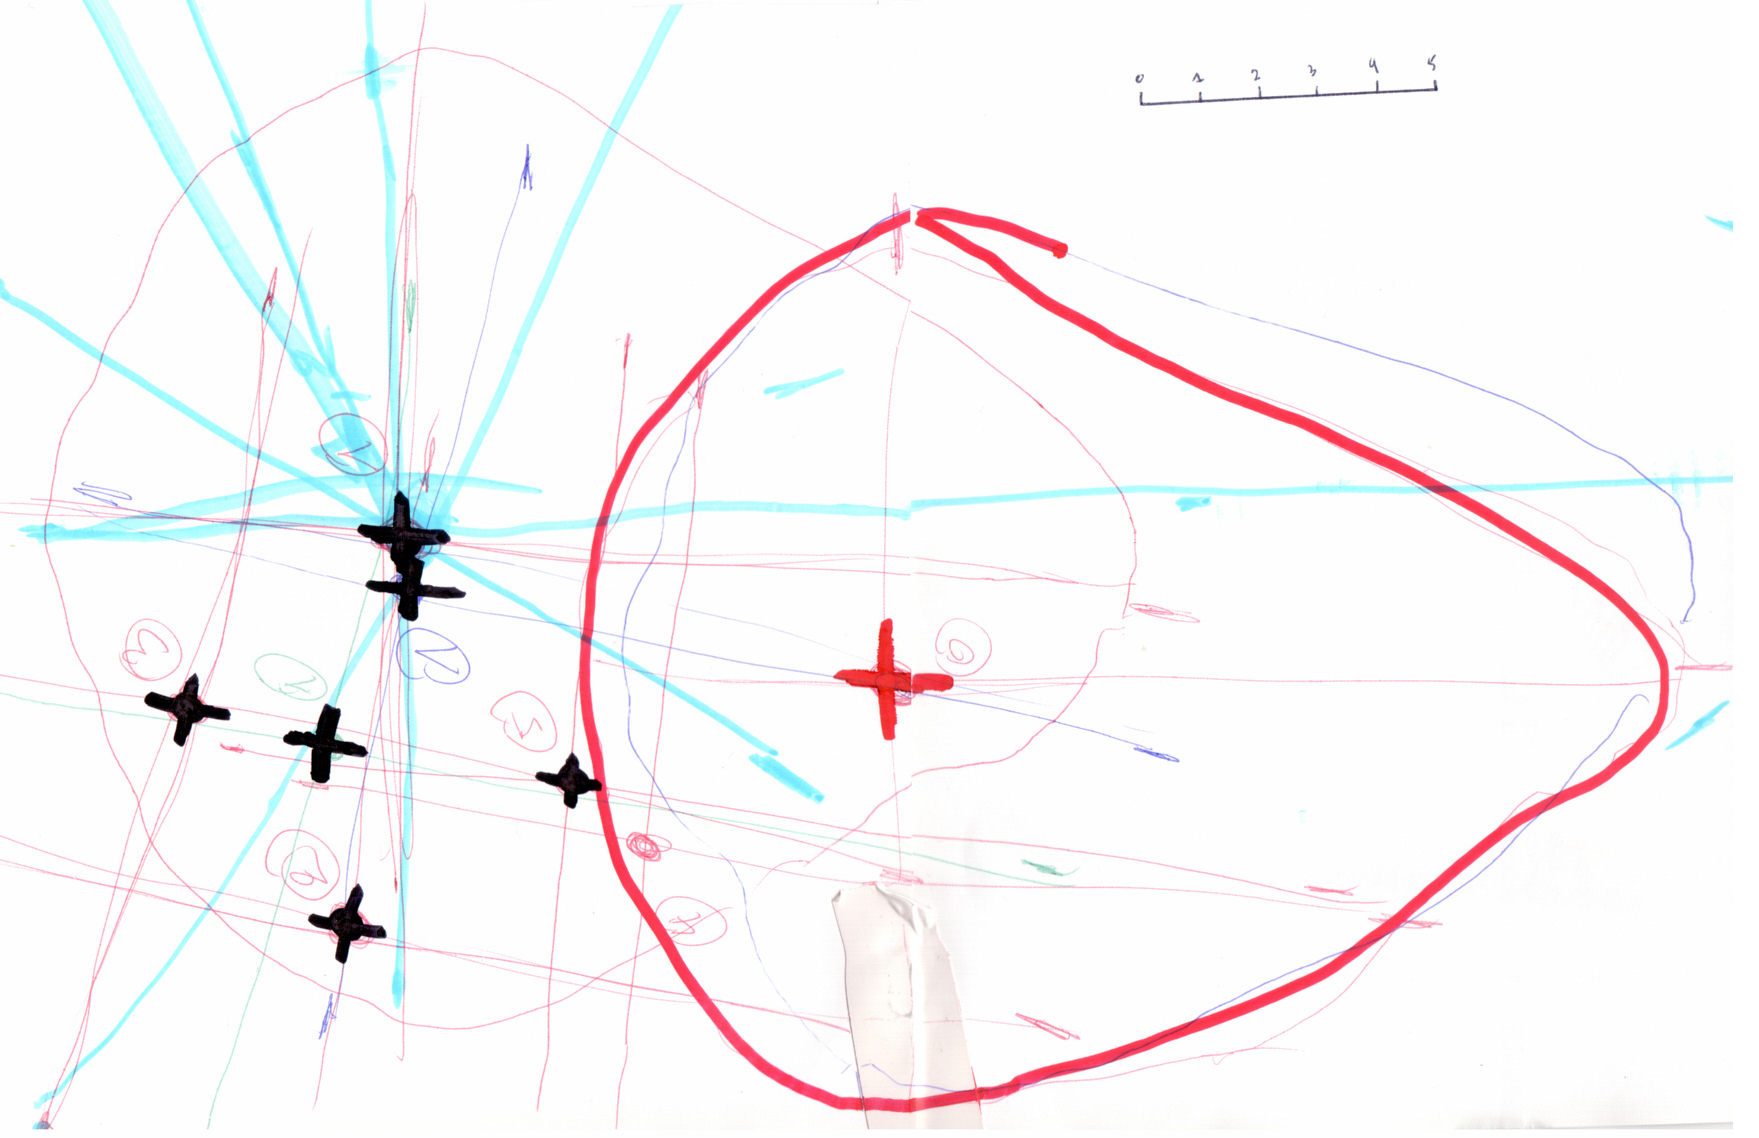
\includegraphics[width=140mm]{resources/meetresultaten.png}
   \caption{Meetresultaten voor grote veelhoeken.}
   \label{fig:resultsLargePolygons}
\end{figure}

\subsection{Tijd}

Het aansturen van de motoren op basis van tijd bleek geen valabel alternatief te zijn. De eerste resultaten gaven procentuele afwijkingen in de grootorde van 10 tot 20\%, zodat een verdere vergelijking met de resultaten voor de omwentelingen totaal overbodig werd. Deze piste werd dan ook verlaten.

\section{Resultaten van de demo}

Tijdens de demo werd gevraagd om een veelhoek van eigen keuze te rijden. We opteerden voor een driehoek met een zijde van 40cm. De afwijking van het startpunt bedroeg ongeveer 10cm.

De tweede veelhoek die opgegeven werd was een tienhoek met een zijde van 20cm. De afwijking van het startpunt bedroeg ongeveer 30cm.

\section{Conclusies}

De resultaten van de demo waren zo sterk afwijkend van de eerder opgemeten waarden tijdens onze testen dat we op zoek moesten gaan naar een andere oorzaak.

We hebben de tienhoek opnieuw meermaals gereden en merkten op dat de afwijking sterk groeide per keer we de veelhoek reden. De eerste keer was de afwijking 3cm, daarna 6cm en 9cm. Bij elke rit viel op dat de wielen meer en meer doorslipten. Dit deed ons kijken naar de kwaliteit van de banden.

De reden bleek de vervuiling van de banden te zijn. Bij elke rit werden de banden vuiler, waardoor de weerstand lager werd, het doorslippen en de daaruit voortvloeiende afwijking groter. Herhaalde testen met proper gemaakte banden leverden opnieuw de nagenoeg foutloze resultaten op. Daarop volgende ritten toonden opnieuw consistent het eerder ervaren vervuiling-en-verval-patroon.

We hadden dit reeds een maal ervaren tijdens onze eerdere testen. Echter nooit was het probleem zo groot. Ook hiervoor hebben we een fout gevonden in onze manier van werken. Het merendeel van de testen waren uitgevoerd op houten banken en niet op de (vuile) vloer. Hierdoor werden bij het merendeel van onze testen de wielen niet zo vuil, met meer consistente resultaten tot gevolg.

We hebben dit probleem en bijhorende (eenvoudige) oplossing post-mortem nog verhaald bij de professoren en mochten onze robot opnieuw laten rijden. Hierbij bleek dat met propere banden onze afwijking de kleinste was van alle deelnemende robots.

Maar dit probleem is wel eigen aan onze robot/ontwerp en we moeten dit beter opnemen in ons project. Daarom zijn we nagegaan hoe het verloop van deze fout evolueert, op zoek naar een maximum, dat dan als correctie kan doorgevoerd worden.

\bigskip
TODO
\bigskip

\appendix

\chapter{Work Breakdown Structure}
\label{appendix:wbs}

\begin{longtable}{r l l c}
\caption{Work Breakdown Structure} \\ [0.5ex]

%This is the header for the first page of the table...
\hline\hline
\# & Omschrijving & Verantwoordelijke & Milestone \\ [0.5ex]
\hline 
\endfirsthead

%This is the header for the remaining page(s) of the table...
\multicolumn{4}{c}{{\tablename} \thetable{} -- Vervolg} \\[0.5ex]
\hline \hline
\# & Omschrijving & Verantwoordelijke & Milestone \\ [0.5ex]
\hline 
\endhead
1	& bepalen optimaal algoritme/verplaatsing	& 					& Demo 1\\
1,1	& codering robot API met tijd/snelheid		& Michiel				& \\
1.2	& codering robot API met omwentelingen		& Ruben				& \\
1.3	& codering tests : tijd/snelheid				& Michiel, Florian 		& \\
1.4	& codering tests : omwentelingen			& Michiel				& \\
1.5	& uitvoeren alle tests, metingen,...			& Ruben, Daniel		& \\
2	& implementatie veelhoek oplossing		& Ruben				& Demo 1 \\
3	& ontwikkeling LCD menu				& Thomas				& \\
4	& verslag voorbereiden					& Christophe			& \\
4.1	& voor demo 1							&					& Demo 1 \\
4.2	& voor demo 2							& 					& Demo 2 \\
4.3	& voor finale demo						&					& Finale \\
5	& ontwikkeling communicatie component		&					& \\		
5.1	& ontwikkeling communicatie thread			&					& \\
5.1.1	& ontwikkeling log kanaal					& Ruben				& Demo 2 \\
5.1.2	& ontwikkeling commando kanaal			& Michiel				& \\
5.2	& ontwikkeling robot agent				&					& \\		
5.2.1	& ontwikkeling log kanaal					& Ruben				& Demo 2 \\
5.2.2	& ontwikkeling commando kanaal			& Michiel				& \\
6	& ontwikkeling model component			& Christophe			& Final \\
7	& ontwikkeling navigator					&					& \\
7.1	& ontwikkeling abstracte navigator			& Christophe			& \\
7.2	& design concrete navigator				&					& \\
7.3	& implementatie concrete navigator			&					& \\
7.4	& testen concrete navigator				&					& \\
8	& ontwikkeling simulator					& Christophe			& \\
9	& ontwikkeling log server					& Michiel, Ruben		& Demo 2 \\
10	& opzetten syslog, file, tail -f mini-client		& Michiel, Ruben		& Demo 2 \\
11	& opzetten database server				& Christophe			& \\
12	& ontwikkeling Fat Client					&					& \\	
12.1	& weergave robot status uit database		& Michiel				& (Demo 2) \\
12.2	& implementatie commando�s				& Michiel				& \\
13	& ontwikkeling SOA						&					& \\
13.1	& opzetten REST service					& Christophe, Ruben 	& \\
13.2	& ontwikkeling web client					& Christophe, Ruben	& \\
14	& ontwikkeling Smart client				& Florian, Thomas		& \\
15	& ontwikkeling zelf-calibratie				& Ruben, Daniel		& \\
16	& controle, vervolledigen unit testen			& Florian				& \\
17	& demo 2 : lijnvolger						& 					& Demo 2 \\
17.1	& onderzoek lichtsensor					& Thomas				& \\
17.2	& implementatie lichtsensor				&					& \\	
17.3	& implementatie lijnvolger				& Thomas, Florian		& \\
18	& demo 2 : muurvolger					& 					& Demo 2 \\
18.1	& onderzoek sonarsensor					& Ruben				& \\
18.2	& implementatie sonarsensor				& Ruben				& \\
18.3	& implementatie muurvolger				&					& \\	
19	& demo 2 : barcode						& 					& Demo 2 \\
19.1	& onderzoek detectie barcodes			& Thomas, Daniel		& \\
19.2	& implementatie barcode					&					& \\	
19.3	& implementatie barcode lezer				&					& \\
\hline
\label{tab:wbs}
\end{longtable}

\chapter{Planning}
\label{appendix:planning}

\begin{figure}[htbp]
\centering
\begin{tikzpicture}
	\begin{ganttchart}[ 
	  y unit title=0.6cm,
	  y unit chart=0.5cm,
	  vgrid,
	  bar height=.5,
	  group right shift=0,
	  group top shift=.6,
	  group height=.3]{22}
\gantttitle{Oktober}{10} 	   	\gantttitle{November}{8} 	    \gantttitle{December}{4} \\
\gantttitlelist{3,10,17,24,31}{2}	\gantttitlelist{7,14,21,28}{2}  \gantttitlelist{5,12}{2} \\
\ganttgroup{1. Beweging}{1}{5} \\
\ganttbar{1.1. API Tijd}{2}{4} \\
\ganttbar{1.2. API Omw.}{2}{4} \\
\ganttbar{1.3. Tijd}{4}{5} \\
\ganttbar{1.4. Omw.}{4}{5} \\
\ganttbar{1.5. tests}{5}{5} \\
\ganttbar{2. Veelhoek}{3}{5} \\
\ganttbar{3. LCD}{2}{5} \\
\ganttmilestone{Demo 1}{5} \ganttnewline
\ganttgroup{4. Verslag}{1}{20} \\
\ganttbar{4.1. Demo 1}{2}{5} \\
\ganttbar{4.2. Demo 2}{8}{12} \\
\ganttbar{4.3. Finaal}{18}{20} \\
\ganttgroup{5. Comm.}{3}{20} \\
\ganttgroup{5.1. Robot}{3}{20} \\
\ganttbar{5.1.1. Log}{3}{11} \\
\ganttbar{5.1.2. Commando}{11}{20} \\
\ganttgroup{5.2. PC}{5}{20} \\
\ganttbar{5.2.1. Log}{5}{11} \\
\ganttbar{5.2.2. Commando}{11}{20} \\
\ganttbar{6. Model}{3}{18} \\
\end{ganttchart}
\end{tikzpicture}
\caption{Planning}
\label{fig:planning}
\end{figure}

\begin{figure}[htbp]
\centering
\begin{tikzpicture}
	\begin{ganttchart}[ y unit title=0.6cm, y unit chart=0.5cm,  vgrid,
	  bar height=.5,
	  group right shift=0,
	  group top shift=.6,
	  group height=.3]{22}
\gantttitle{Oktober}{10} 	   	\gantttitle{November}{8} 	    \gantttitle{December}{4} \\
\gantttitlelist{3,10,17,24,31}{2}	\gantttitlelist{7,14,21,28}{2}  \gantttitlelist{5,12}{2} \\
\ganttgroup{7. Navigator}{5}{18} \\
\ganttbar{7.1. Abstract}{5}{11} \\
\ganttbar{7.2. Design}{11}{18} \\
\ganttbar{7.3. Impl.}{13}{18} \\
\ganttbar{7.4. Tests}{15}{18} \\
\ganttbar{8. Simulator}{3}{13} \\
\ganttbar{9. Log server}{5}{11} \\
\ganttbar{10. Syslog}{7}{10} \\
\ganttbar{11. DB server}{7}{10} \\
\ganttgroup{12. Fat client}{9}{16} \\
\ganttbar{12.1. Status}{9}{14} \\
\ganttbar{12.2. Commando}{10}{16} \\
\ganttgroup{13. SOA}{9}{12} \\
\ganttbar{13.1. REST}{9}{11} \\
\ganttbar{13.2. web client}{10}{12} \\
\ganttbar{14. Smart client}{12}{18} \\
\ganttbar{15. Calibratie}{12}{18} \\
\ganttbar{16. Unit tests}{2}{18} \\
\ganttgroup{17. Lijnvolger}{5}{10} \\
\ganttbar{17.1. Onderzoek}{5}{8} \\
\ganttbar{17.2. Sensor}{7}{9} \\
\ganttbar{17.3. Impl.}{9}{10} \\
\ganttgroup{18. Muurvolger}{5}{10} \\
\ganttbar{18.1. Onderzoek}{5}{8} \\
\ganttbar{18.2. Sensor}{7}{9} \\
\ganttbar{18.3. Impl.}{9}{10} \\
\ganttgroup{19. Barcode}{5}{10} \\
\ganttbar{19.1. Onderzoek}{5}{8} \\
\ganttbar{19.2. Detectie}{7}{9} \\
\ganttbar{19.3. Impl.}{9}{10} \\
\ganttmilestone{Demo 2}{10} \ganttnewline
\ganttmilestone{Finale Demo}{18} \ganttnewline
\ganttbar{20. Finaal verslag}{19}{20} \\
\end{ganttchart}
\end{tikzpicture}
\caption{Planning (vervolg)}
\label{fig:planning2}
\end{figure}

\chapter{Klasse Diagrammen}
\label{appendix:classdiagrams}

\chapter{Tijdsregistratie}
\label{appendix:tijdsregistratie}



\end{document}
